\documentclass{standalone}
\usepackage[T1]{fontenc}
\usepackage[utf8]{inputenc}
\usepackage{pgf,tikz}
\usepackage{pgfplots}
\pgfplotsset{compat=1.9}

\begin{document}

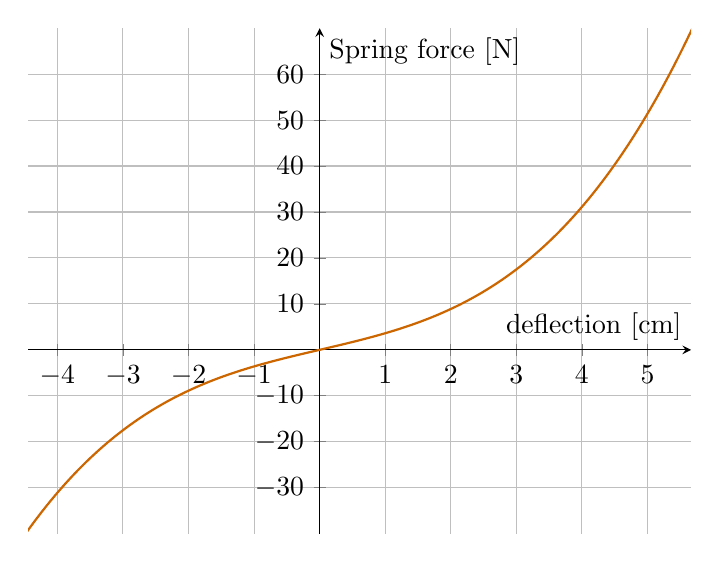
\begin{tikzpicture}[%
  node distance=2cm,
  block/.style={rectangle, draw, minimum width=14mm, minimum height=10mm},
  ]
  \begin{axis}[%
    width=10cm,
    height=8cm,
    axis lines=middle,
    xlabel={deflection [cm]},
    ylabel={Spring force [N]},
    grid=both,
    ymin=-40,
    ymax=70,
    ytick={-30,-20,...,60},
    xtick={-5,-4,...,6},
    ]
    \addplot [orange!80!black, thick, no marks, smooth, domain=-5:6, samples=100] {20/6 * x +  60/pow(6, 3) * pow(x, 3)};
  \end{axis}
\end{tikzpicture}
\end{document}
